    	\section{Continuous-Time Quantum Walk}\label{contwalk}
    	        The continuous-time random walk model on a graph is a Markov process where transitions have a fixed probability per unit time $\gamma$ of moving to adjacent vertices, firstly introduced by \cite{montrollweiss1965}. Consider a graph $G$ with $N$ vertices and no self-loops, this walk can be defined by the linear differential equation that describes the probability of jumping to a connected vertex in any given time \textcolor{red}{pode colocar G(V,E) e depois especificar que (i,j) é uma aresta}
    	        \begin{equation}
    	            \frac{dp_i(t)}{dt} = \gamma \sum_j L_{ij} p_j(t), \label{contWalk}
    	        \end{equation}
    	        where $L$ is the Laplacian defined as $L = A - D$. $A$ is the adjacency matrix that represents each vertex connection, given by
    	        \begin{equation}
    	           A_{ij} = \begin{cases} 1, & \mbox{if } (i,j)\in G \\ 0, & \mbox{otherwise,} \end{cases}
    	        \end{equation}
    	        and D is the diagonal matrix $D_{jj} = deg(j)$ corresponding to the degree\footnote{The degree of a vertex refers to the number of edges that it is connected to.} of a vertex $j$.
    	        
                In the quantum case, the nodes are quantum states that form the basis for the Hilbert space. The continuous-time quantum walk model will also be described by a differential equation, the Schrödinger equation
                \begin{equation}
                    i\hbar \frac{d\ket{\Psi(t)}}{dt} = \hat{H} \ket{\Psi(t)}, \label{shrodinger}
                \end{equation}
                where $\hat{H} = -\gamma L$ is the Hamiltonian of the system. More explicitly,
                \begin{equation}
                    \hat{H}_{ij} = \begin{cases} 
                            deg(j)\gamma, & \mbox{if } i= j; \\ 
                            -\gamma, & \mbox{if } i\neq j\mbox{ and adjacent};\\
                            0, & \mbox{if } i\neq j\mbox{ and not adjacent}.
                        \end{cases}.
                        \label{Hamilt}
                \end{equation}\par
                A general state of a system $\ket{\Psi(t)}$ can be written as a function of it's complex amplitudes \textcolor{red}{acredito que seja contrária a relação, as amplitudes que são descritas pelo estado através da equação 28}
                \begin{equation}
                    q_i = \braket{i|\Psi(t)},
                \end{equation}
                which means \ref{shrodinger} can be rewritten as 
                \begin{equation}
                     i\hbar \frac{dq_i(t)}{dt} = \sum_j \hat{H}_{ij} q_j(t).
                \end{equation}
                This highlights the similarities between the Schrödinger equation and \ref{contWalk}. One of the main differences is the complex phase $i$, which will result in a very different behaviour. \textcolor{red}{você pode dizer que a 29 é uma quantização da 24}\par
                Setting $\hbar = 1$ and solving the differential equation results in the evolution operator of this walk \textcolor{red}{acho que podemos ajustar, talvez a equação 32 deva subir, porque ela que é solução da equação diferencial}%mencionar redimens. devido ao planck modificado
            	\begin{equation}
            	    U(t) = e^{-iHt} = e^{i(-\gamma L)t} = e^{-i\gamma(A+D)t}
            	\end{equation}
            	In the regular graph case, where $D$ is simply the degree of the whole graph multiplied by the identity matrix, $A$ and $D$ will commute, meaning that the evolution operator can be written in terms of the adjacency matrix \textcolor{red}{ficou muito bom isso daqui}
            	\begin{equation}
            	   U(t) = e^{-i\gamma A t + i\gamma D t} = e^{-i\gamma A t} e^{i\gamma D t} = \phi(t) e^{-i\gamma A t} 
            	\end{equation}
            	since the degree matrix becomes a global phase.
            	%that can be verified by expanding the %exponential function in Taylor series.
            	%Demonstrar com eq dif ordinarias de variaveis separaveis.
            	Applying this operator to an initial condition $\Psi(0)$, will give the state of the system at a time $t$
                \begin{equation}
                    \ket{\Psi(t)} = U(t)\ket{\Psi(0)}.
                \end{equation}\par
                Considering a uni-dimensional quantum system, each vertex will have at most 2 other neighboring vertices, reducing equation \ref{Hamilt} to
                \begin{equation}
                \hat{H}_{ij} = \begin{cases} 
                            2\gamma, & \mbox{if } i= j; \\ 
                            -\gamma, & \mbox{if } i\neq j\mbox{ and adjacent};\\
                            0, & \mbox{if } i\neq j\mbox{ and not adjacent}.
                        \end{cases}
                \end{equation}\par
                For a more detailed visualization, this quantum walk model was coded in python and figure \ref{fig:contdist0} was obtained setting the transition rate to $\gamma=\frac{1}{2\sqrt{2}}$ the initial condition to $\ket{\Psi(0)} = \ket{0}$ \textcolor{red}{cortou a figura}
                
                \begin{figure}[!h]
                    \centering
                    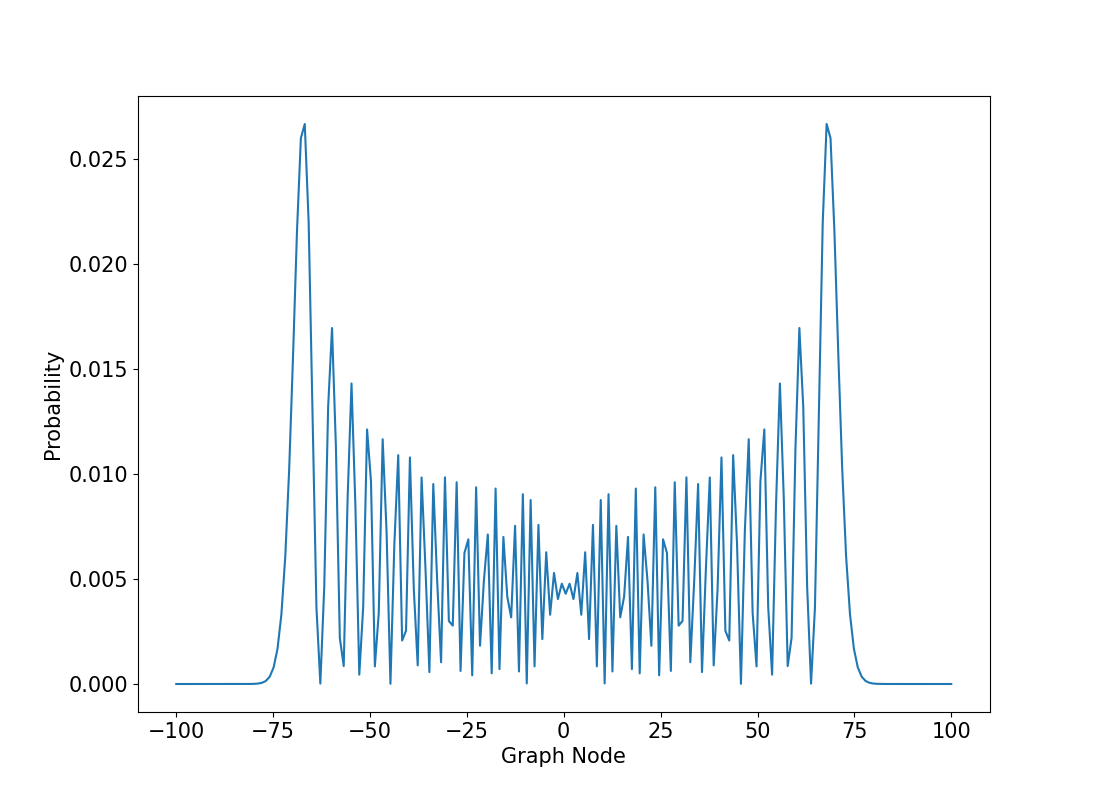
\includegraphics[scale=0.40]{img/ContQuantumWalk/ctqwSinglePsi0.png}
                    \caption{Probability distribution for the continuous-time quantum walk on a line, at t = 100, with initial condition $\ket{\Psi(0)}=\ket{0}$ and $\gamma=\frac{1}{2\sqrt{2}}$.} 
                    \label{fig:contdist0}
                \end{figure}
                
            A brief look at figure \ref{fig:contdist0} reveals several similarities to the coined quantum walk model of figure \ref{fig:coinedwalk3}. Both have two peaks away from the origin and low probability near the origin.
             However, in the previous quantum walk, these characteristics were altered as a function of the chosen coin and initial condition, whereas in this case different values of $\gamma$ will influence the probability distribution. For example, a lower value of $\gamma$ will limit the spread of the probability distribution, as is shown in figure \ref{fig:contdist1}. \textcolor{red}{você pode dizer que o desvio padrão é proporcional ao $\gamma$ também}
                \begin{figure}[!h]
                    \centering
                    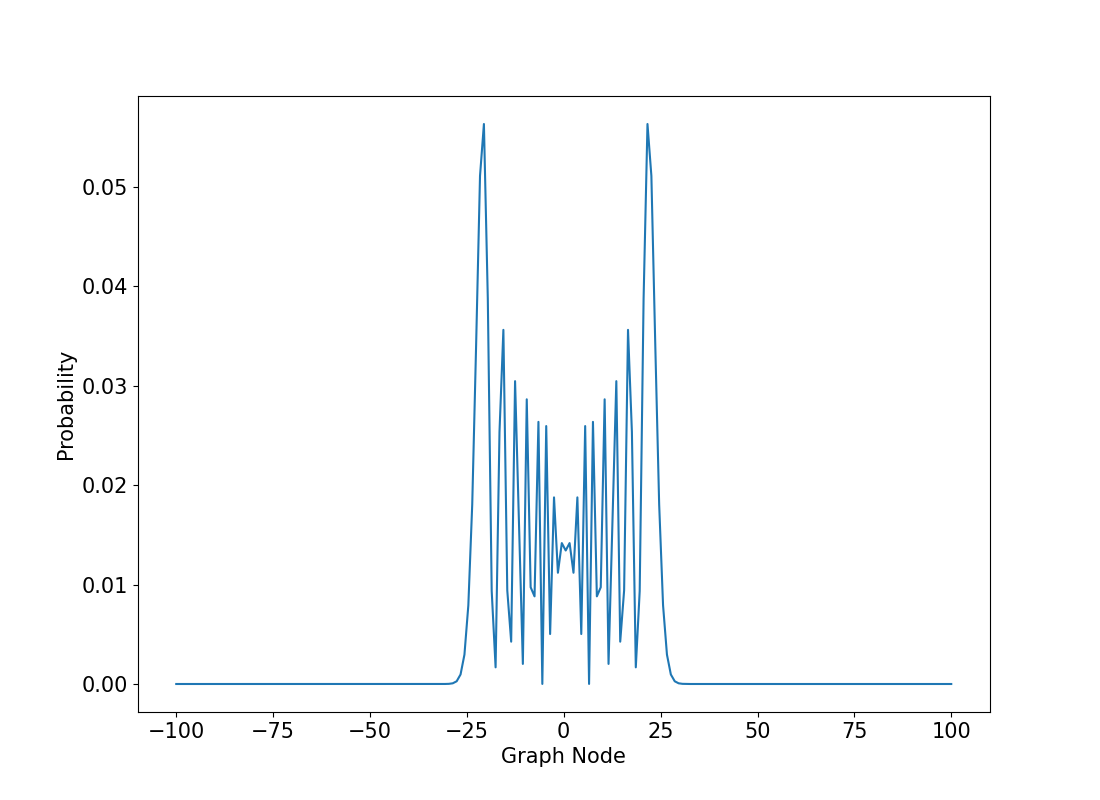
\includegraphics[scale=0.40]{img/ContQuantumWalk/ctqwSinglePsi0LowerGamma.png}
                    \caption{Probability distribution for the continuous-time quantum walk on a line, after 100 steps, with initial condition $\ket{\Psi(0)}=\ket{0}$ and $\gamma=\frac{1}{6\sqrt{2}}$.} 
                    \label{fig:contdist1}
                \end{figure}
                
                \begin{figure}[!h]
                    \centering
                    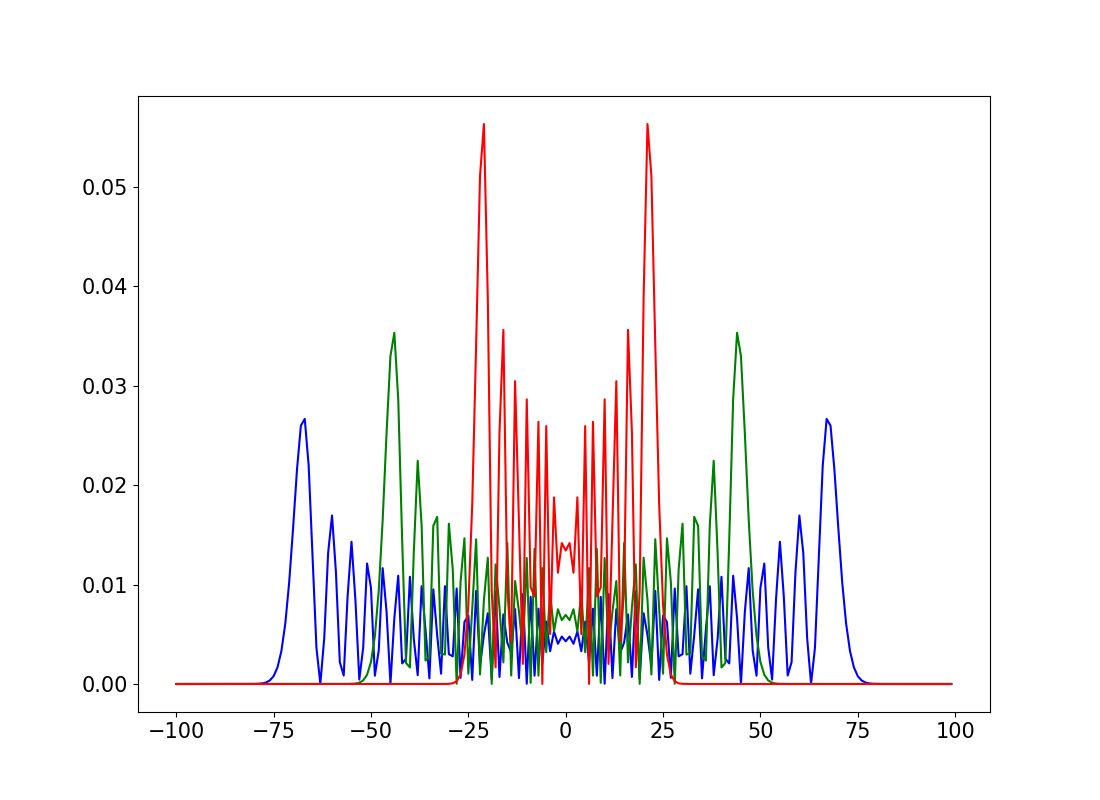
\includegraphics[scale=0.40]{img/ContQuantumWalk/ctqwMultipleGamma.png}
                    \caption{Temporary} 
                    \label{fig:contdist1}
                \end{figure}
                
            Moreover, the effects of altering the initial condition will also differ in the continuous-time example. For example, setting the initial condition to the balanced superposition of states $\ket{0}$ and $\ket{1}$ has no effect on the overall pattern of the probability distribution as can be seen in figure \ref{fig:contdist2}. Both peaks still are still present and at the same distance from the origin, with intermediate amplitudes being attenuated relative to figure \ref{fig:contdist0}. This behaviour is in contrast with the discrete-time case, where a change in the initial condition would dictate the number of peaks and where they would appear.
            
                \begin{figure}[!h]
                    \centering
                    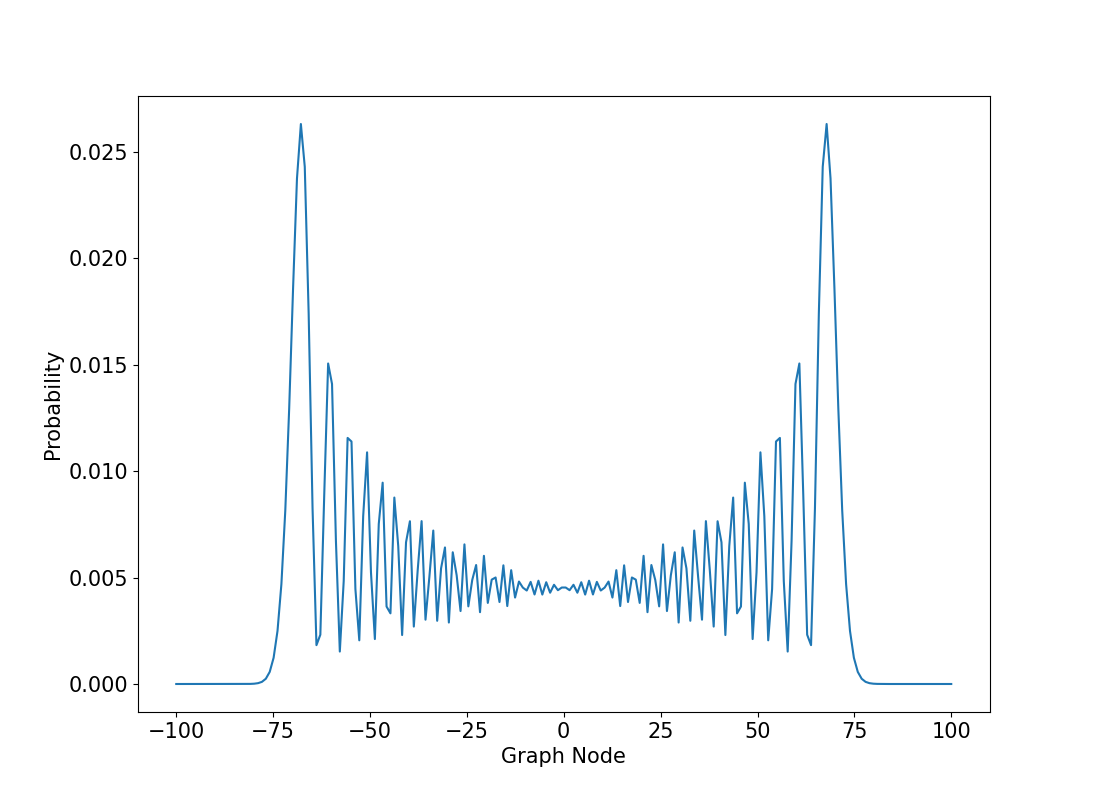
\includegraphics[scale=0.40]{img/ContQuantumWalk/ctqwSingleSup.png}
                    \caption{Probability distribution for the continuous-time quantum walk on a line, after 100 steps, with initial condition $\ket{\Psi(0)}=\frac{\ket{0}+\ket{1}}{\sqrt{2}}$ and $\gamma=\frac{1}{2\sqrt{2}}$.} 
                    \label{fig:contdist2}
                \end{figure}
                
                \begin{figure}[!h]
                    \centering
                    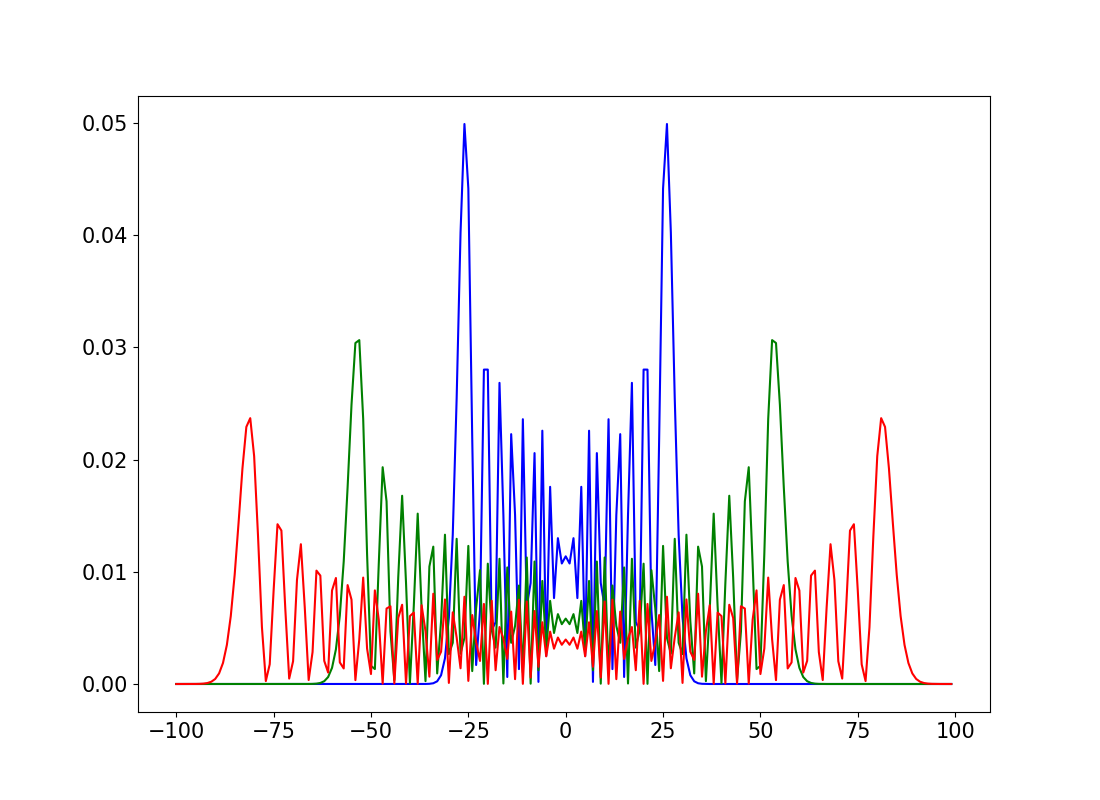
\includegraphics[scale=0.40]{img/ContQuantumWalk/ctqwMultipleTime.png}
                    \caption{Temporary} 
                    \label{fig:contdist2}
                \end{figure}
                
             \textcolor{red}{precisa de um fechamento aqui também, alguns resultdos e referências mais talvez}
             
                \clearpage
                
